\section{System Overview}
Our system mainly consists of a set of processes which receive events, process them and forward to next processes. We use the term adapters for special processes which receive events from out side systems. These processes and adapters forms a graph which represents the way a given event stream being processed within the system. Our current implementation does not support fault tolarance and have adapted topoloy concept from twitter storm\cite{twitterStorm} and cluster concept from Yahoo S4\cite{neumeyer2010s4}. Rest of this section further describes this concept at a user level. In the next section we provide a detail explanation about how we have make this interprocess communication efficient. 
\subsection{Process Graph}
A Process graph (Figure \ref{processgraph}) mainly consists of the adapters, processes which does the processing logic and their interaction patterns. Adapters receive events from out side systems and forward them to other processes. Processes process events according to a given logic and emits the generated events either to other processes or to out side systems. 

\begin{figure}[!t]
	\centering
	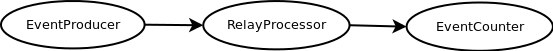
\includegraphics[width=3.0in]{processgraph.png}
	\caption{Process Graph}
	\label{processgraph}
\end{figure}

\subsection{Runtime Graph}
When the system is deployed, there can be many instances of one process to handle higher loads making system scalable. Figure \ref{runtimegraph} shows possible runtime graph for above process graph. Here each parent process instance sends events to two child process instances. However in this case parent process instance has to pick a child process instance to send the message as well. One way of handling this problem is to pick a random node. Other way is to send messages with same key to same child process instance. 

\begin{figure}[!t]
        \centering
        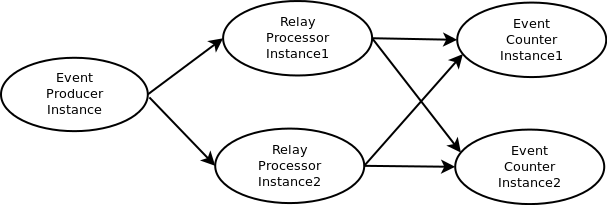
\includegraphics[width=3.0in]{runtimegraph.png}
        \caption{Runtime Graph}
        \label{runtimegraph}
\end{figure}

\subsection{API}
In this section, we explain our API which can be used to define custom events, processes and adapters. We provide clear interfaces to abstract out all the communication complexities from application developers.

\definecolor{dkgreen}{rgb}{0,0.6,0}
\definecolor{gray}{rgb}{0.5,0.5,0.5}
\definecolor{mauve}{rgb}{0.58,0,0.82}

\lstset{frame=tb,
  language=Java,
  aboveskip=3mm,
  belowskip=3mm,
  showstringspaces=false,
  columns=flexible,
  basicstyle={\small\ttfamily},
  numbers=none,
  numberstyle=\tiny\color{gray},
  keywordstyle=\color{blue},
  frame=single,
  breaklines=true,
  breakatwhitespace=true,    
  tabsize=2
}

\begin{lstlisting}
public interface Event {
    String getKey();
    void serialize(DataOutput dataOutput);
    void parse(DataInput dataInput);
}

public interface Element {
    void initialise(Container container,
            Map<String,String> parameters);
}

public interface Adaptor extends Element {
    void start();
}

public interface Processor extends Element {
    void onEvent(Event event);
}
\end{lstlisting}

 The Event interface has a method to get the key for a given event. This key is used in sending messages to next processes as described earlier. Parse and serialize methods of event interface are used to direcly serialize the event attributes to underline streams. When implementing these methods deveopers can define attibute serializing order in serialize method and use same order at the parse method to avoid meta data passing with the binary format. Process interface has a method called onEvent which underline framework invokes when it receives an event to that process. The start method of the adapter interface is invoked by the framework and that can be used to pull events from out side systems onces the system starts. At the initilization time both processes and adapters receive the container which can be used to send events to other processes.
 
 \subsection{Deployment}

As shown in Figure \ref{deployment}, a deployment of the system consists of a manager node and a set of worker nodes. Worker nodes are grouped into clusters so that the application users can specify to which clusters each processes needs to get deployed. Manager node process applications, deploy them to worker nodes and initiate the processing by starting the adapters.

\begin{figure}[!t]
        \centering
        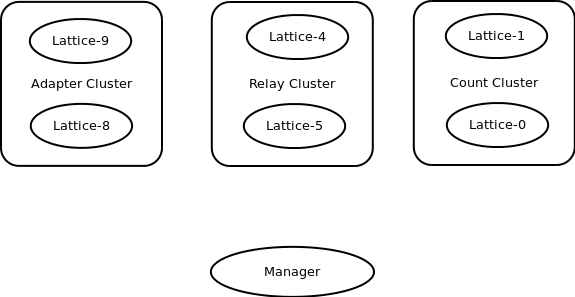
\includegraphics[width=3.0in]{deployment.png}
        \caption{Deployment}
        \label{deployment}
\end{figure}

\subsection{Application Developement}

An application specifies the runtime graph to process a pirticular event stream. Therefore an appication mainly consists of a set of processes, adapters and events and their interactions. Processes, adapters and events can be developed by implementing the respective interfaces as shown above. Then the interactions can be specified using a json file. 

\lstinputlisting{runtimegraph.json}

As shown above, the \textit{instances} parameter can be used to specify the required number of instances to be deployed. The \textit{receivers} parameter is used specify from which process it expects to receive messages and how the sending process should distribute the events among instances. The \textit{key} type indicates that events with same key must be received for same instance. Finally users can deploy the application to manager which process them and deploys to workers.






 
